% \begin{figure}
%     \centering
%     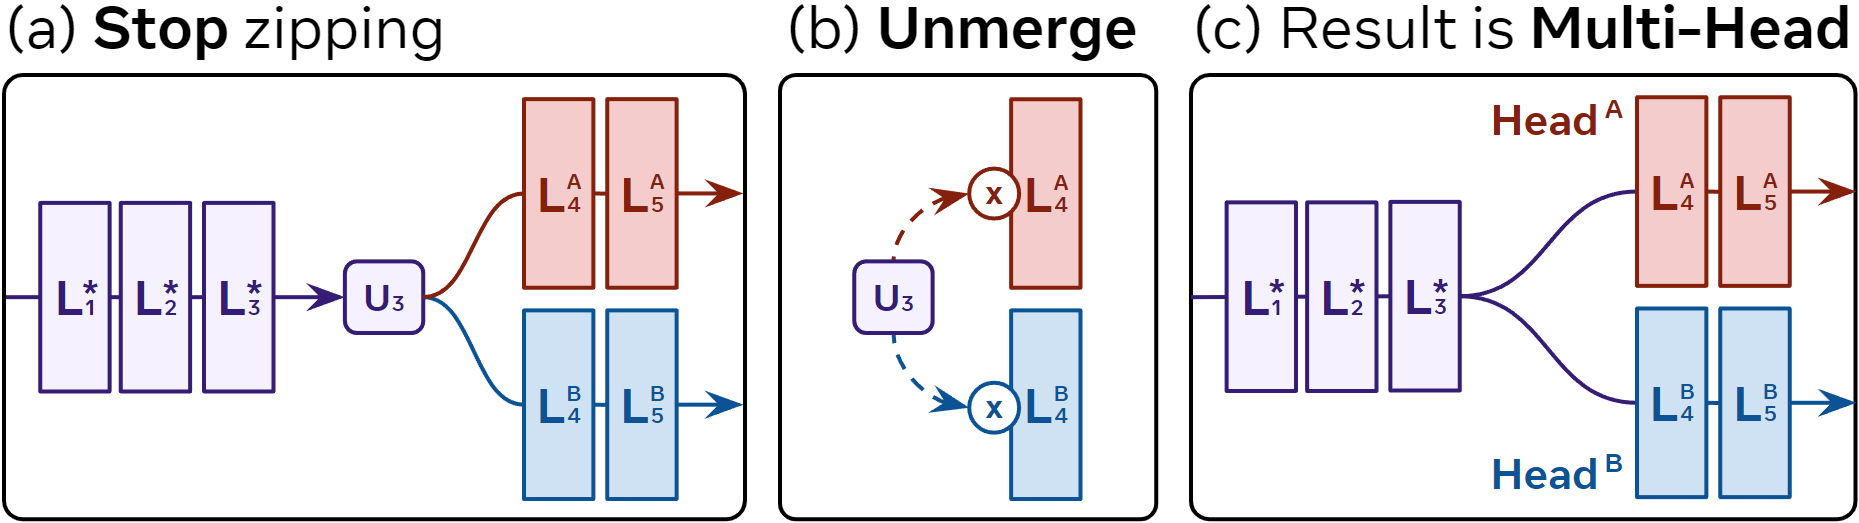
\includegraphics[width=\linewidth]{figures/imgs/partial_zip.png}
%     \caption{
%         {\bf Partial Zip.} 
%         If we stop zipping early (a), we can create a multi-head model that can perform multiple tasks. All we need to do is apply the last unmerge from zip propogation (Fig.~\ref{fig:zip_prop}) to the inputs of the first unmerged layer in each model (b), and we get a model with multiple heads (c).
%     }
%     \label{fig:partial_zip}
% \end{figure}